\section{Durchführung}
\label{sec:Durchführung}

\subsection{Versuchsaufbau}
\label{sec:Versuchsaufbau}
%\begin{figure}
%	\centering
%	\caption{Schematische Darstellung des Versuchsaufbaus \cite{anleitung}.}
%	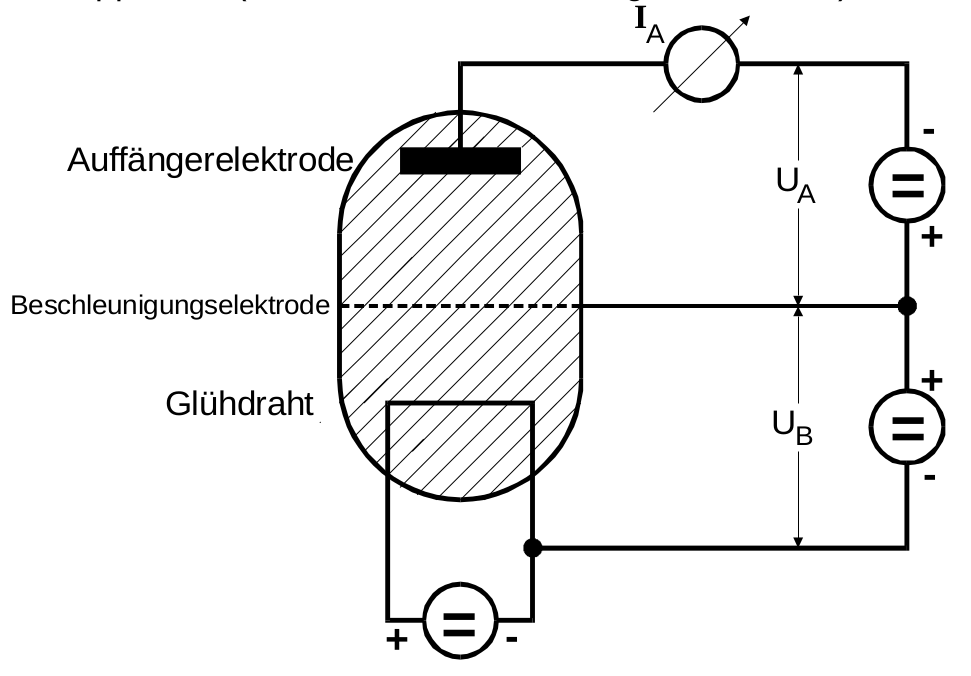
\includegraphics{Bilder/aufbau.png}
%	\label{fig:aufbau}
%\end{figure}
%
%\begin{figure}
%	\centering
%	\caption{Schematische Darstellung der Quelle zur Erzeugung radioaktiven Isotopen \cite{anleitung}.}
%	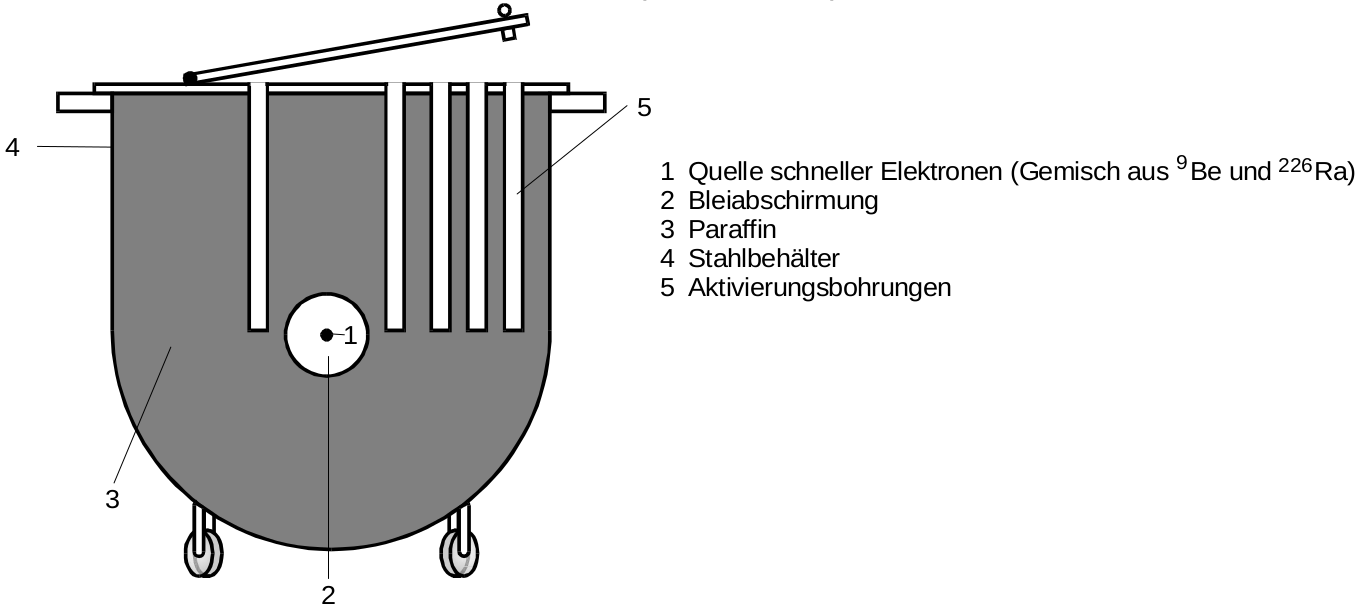
\includegraphics{content/toepfchen.png}
%	\label{fig:kochen}
%\end{figure}
%
Der Versuchsaufbau -- wie in Abbildung \ref{fig:aufbau} dargestellt -- besteht im Wesentlichen 
aus einem zerfallenden radioaktiven Isotop und einem Geiger-Müller-Zählrohr, welches die 
zerfallenden Kerne misst.
Das Geiger-Müller-Zählrohr ist entspricht einer mit Gas gefüllten Röhre. Trifft ein $\beta$-
oder $\gamma$- Teilchen auf ein Gasteilchen wird dieses ionisiert und kann aufgrund einer
anliegenden Spannung an der Röhre gemessen werden.
Dabei werden die gemessenen Zerfälle pro Messzeitintervall, welches am Zeitgeber einstellbar 
ist, an den Zählern 1 und 2 angezeigt. Nach jedem Messvorgang wird der Zähler umgeschaltet und 
der vorherige Wert auf dem aktuellen Zähler wird überschrieben. Der Versuchsaufbau ist mit
einer Blei-Abschirmung ausgestattet um die radioaktive Strahlung abzuschirmen.

Zur Erzeugung der radioaktiven Isotope wird das Objekt in Abbildung \ref{fig:kochen} verwendet.
Hierbei werden stabile Kerne mit niederenergetischen Neutronen beschossen. 
Da die Neutronen ihre Energie durch elastische Stöße an die Kerne übergeben und die maximale
Energie bei gleichen Massen der Stoßpartner erreicht wird, werden die Neutronen in einem 
Paraffinmantel gebremst, bis sie die optimale Energie besitzen.


\subsection{Versuchsbeschreibung}
\label{sec:Versuchsbeschreibung}
Vor Beginn jeder Messung muss der XY-Schreiber geeignet kalibriert werden.
Das verwendete Millimeterpapier lässt sich hierbei elektrostatisch auf dem XY-Schreiber fixieren.
Bevor ein Signal auf die Eingänge des XY-Schreibers gegeben wird, muss der Nullpunkt der Messung festgelegt werden. Dazu wird mit den beiden "Zero"-Knöpfen der Messskalen der Schreibkopf mit etwas Abstand zum Rand in der linken, unteren Ecke des Millimeterpapiers platziert.
Zur Justierung der Empfindlichkeit der beiden Eingänge wird der Versuch ohne Aufzeichnung einer Messkurve durchgeführt. Dafür werden die zu messenden Signale auf die jeweiligen Eingänge des XY-Schreibers gegeben.
Die Empfindlichkeit beider Eingänge wird so geregelt, dass die jeweiligen maximalen und minimalen Werte mit etwas Abstand zum Rand liegen.
Für jede Messung können nun Messkurven aufgezeichnet werden. Hierfür wird die Schutzhülle vom Schreibkopf des XY-Schreibers entfernt, und der Schreibkopf vorsichtig auf das Millimeterpapier gesetzt.\\
Nach dem Abschluss jeder Messreihe ist es notwendig, die x-Achse zu skalieren. Hierfür wird das auf die Y-Achse aufgegebene Signal entfernt und die Messung wird bezüglich des Signals auf dem X-Eingang wiederholt. Der Schreibkopf wird hierfür nicht auf das Millimeterpapier gesetzt.
In regelmäßigen Abständen der gemessenen Spannung am Voltmeter werden Zwischenwerte auf der X-Achse markiert und die zugehörigen Spannungen notiert.

Zur Messung der integralen Energieverteilung der beschleunigten Elektronen wird der Auffängerstrom $I_\mathrm{A}$ in Abhängigkeit der Bremsspannnung $U_\mathrm{A}$ bei konstanter Beschleunigungsspannung $U_\mathrm{B}=\SI{11}{\volt}$ gemessen. Der Auffängerstrom wird hierfür auf den Y-Eingang des XY-Schreibers aufgegeben und die Bremsspannung auf den X-Eingang. Die Bremsspannung wird über die anliegende gesteuerte Gleichspannungsquelle hierbei von $\SI{0}{\volt}$ bis $\SI{11}{\volt}$ variiert.
Die Messung wird einmal bei Zimmertemperatur und einmal bei etwa $150^\circ C$ durchgeführt.
Während der Messung soll die Temperatur im Versuchsaufbau möglich konstant gehalten werden. Dafür wird die Temperatur permanent am elektronischen Thermometer abgelesen und der Heizgenerator entsprechend nachgeregelt.

Zur Aufnahme der Franck-Hertz-Kurve wird die Temperatur im Versuchsaufbau auf den maximal möglichen Wert des vorliegenden Versuchaufbaus von etwa $180^\circ C$ erhöht. Die Bremsspannung wird hierfür permanent auf $\SI{1}{\volt}$ gestellt und die Beschleunigungsspannung von $\SI{0}{\volt}$ bis $\SI{60}{\volt}$ über die gesteuerte Gleichspannungsquelle variiert.
Die variable Beschleunigungsspannung wird auf den X-Eingang und mittels des Pikoamperemeters eine Spannung proportional zum Auffängerstrom $I_\mathrm{A}$ auf den Y-Eingang des XY-Schreibers aufgegeben.

Zur Bestimmung der Ionisatiosnspannung von Quecksilber wird die Innentemperatur des Aufbaus auf etwa $100^\circ C$ geregelt, der Auffängerstrom wird hierbei auf den Y-Eingang gegeben.
An den X-Eingang wird die Beschleunigungsspannung $U_\mathrm{B}$ aufgegeben. Die Bremsspannung ist hierbei konstant $U_\mathrm{A}=\SI{-30}{\volt}$.
